%% This is file `elsarticle-template-1-num.tex',
%%
%% Copyright 2009 Elsevier Ltd
%%
%% This file is part of the 'Elsarticle Bundle'.
%% ---------------------------------------------
%%
%% It may be distributed under the conditions of the LaTeX Project Public
%% License, either version 1.2 of this license or (at your option) any
%% later version.  The latest version of this license is in
%%    http://www.latex-project.org/lppl.txt
%% and version 1.2 or later is part of all distributions of LaTeX
%% version 1999/12/01 or later.
%%
%% The list of all files belonging to the 'Elsarticle Bundle' is
%% given in the file `manifest.txt'.
%%
%% Template article for Elsevier's document class `elsarticle'
%% with numbered style bibliographic references
%%
%% $Id: elsarticle-template-1-num.tex 149 2009-10-08 05:01:15Z rishi $
%% $URL: http://lenova.river-valley.com/svn/elsbst/trunk/elsarticle-template-1-num.tex $
%%
\documentclass[preprint,12pt]{elsarticle}

%% Use the option review to obtain double line spacing
%% \documentclass[preprint,review,12pt]{elsarticle}

%% Use the options 1p,twocolumn; 3p; 3p,twocolumn; 5p; or 5p,twocolumn
%% for a journal layout:
%% \documentclass[final,1p,times]{elsarticle}
%% \documentclass[final,1p,times,twocolumn]{elsarticle}
%% \documentclass[final,3p,times]{elsarticle}
%% \documentclass[final,3p,times,twocolumn]{elsarticle}
%% \documentclass[final,5p,times]{elsarticle}
%% \documentclass[final,5p,times,twocolumn]{elsarticle}

%% if you use PostScript figures in your article
%% use the graphics package for simple commands
%% \usepackage{graphics}
%% or use the graphicx package for more complicated commands
%% \usepackage{graphicx}
%% or use the epsfig package if you prefer to use the old commands
%% \usepackage{epsfig}

%% The amssymb package provides various useful mathematical symbols
\usepackage{amssymb} %for stylish bullet points(math symbols)
%% The amsthm package provides extended theorem environments
%% \usepackage{amsthm}

%% The lineno packages adds line numbers. Start line numbering with
%% \begin{linenumbers}, end it with \end{linenumbers}. Or switch it on
%% for the whole article with \linenumbers after \end{frontmatter}.
\usepackage{lineno}
\usepackage{hyperref}
\usepackage{amsmath, mathdots, paralist}
\usepackage{float}
\usepackage{graphicx} %for inserting images
\usepackage{tabularx} %for tables
\usepackage{ltablex}
\usepackage{array} %for changing row height
\usepackage{enumitem} %for changing spacing around itemize

\usepackage{xpatch}

% Patching the \hrule\vskip12pt out .. do it twice!!!
\makeatletter
\xpatchcmd{\pprintMaketitle}{%
  \hrule\vskip12pt%
}{}{\typeout{Success}}{}
\makeatother

% Customizing footer
\makeatletter
\def\ps@pprintTitle{%
 \let\@oddhead\@empty
 \let\@evenhead\@empty
 \def\@oddfoot{\leftline{\textit{GSoC KDE 2018 \hspace{115mm}\today}}}
 \let\@evenfoot\@oddfoot
 }
\makeatother

\usepackage[left=2cm, right=2cm, top=2.5cm, bottom=2cm, footskip=1cm]{geometry}


%% natbib.sty is loaded by default. However, natbib options can be
%% provided with \biboptions{...} command. Following options are
%% valid:

%%   round  -  round parentheses are used (default)
%%   square -  square brackets are used   [option]
%%   curly  -  curly braces are used      {option}
%%   angle  -  angle brackets are used    <option>
%%   semicolon  -  multiple citations separated by semi-colon
%%   colon  - same as semicolon, an earlier confusion
%%   comma  -  separated by comma
%%   numbers-  selects numerical citations
%%   super  -  numerical citations as superscripts
%%   sort   -  sorts multiple citations according to order in ref. list
%%   sort&compress   -  like sort, but also compresses numerical citations
%%   compress - compresses without sorting
%%
%% \biboptions{comma,round}

\biboptions{sort&compress}


\journal{GSoC KDE 2018}

\begin{document}

\begin{frontmatter}

%% Title, authors and addresses

%% use the tnoteref command within \title for footnotes;
%% use the tnotetext command for the associated footnote;
%% use the fnref command within \author or \address for footnotes;
%% use the fntext command for the associated footnote;
%% use the corref command within \author for corresponding author footnotes;
%% use the cortext command for the associated footnote;
%% use the ead command for the email address,
%% and the form \ead[url] for the home page:
%%
%% \title{Title\tnoteref{label1}}
%% \tnotetext[label1]{}
%% \author{Name\corref{cor1}\fnref{label2}}
%% \ead{email address}
%% \ead[url]{home page}
%% \fntext[label2]{}
%% \cortext[cor1]{}
%% \address{Address\fnref{label3}}
%% \fntext[label3]{}

\title{One Step Closer to Version 1.0}

%% use optional labels to link authors explicitly to addresses:
%% \author[label1,label2]{<author name>}
%% \address[label1]{<address>}
%% \address[label2]{<address>}

\author{Rohit Das}

\address{ \textbf{Email ID}: rohit.das950@gmail.com}
\address{ \textbf{Freenode IRC Nick}: mouri11}
\address{ \textbf{Location}: Serampore, West Bengal, India UTC+5:30}

\end{frontmatter}

%%
%% Start line numbering here if you want
%%
% \linenumbers

%% main text
\section{Motivation}
\label{S:1}

{GCompris is a software suite comprising educational software for children aged 2 to 10. Protected under the GNU General Public License, GCompris is free for developers to work with and contribute to. Having more than 137 activities, developers old and new can have their hands full with fun things to play around. Hence, GCompris is not only educational for the kids, but also for their creators.}

{Teaching kids and making them more imaginative is what GCompris aims at, and I intend to help with the process of its development. Since GCompris was originally written in GTK+, there are many activities to work with, from porting old ones, to completing and creating activities anew in Qt-Quick. The activity I intend to work on is: \textit{Analog Electricity}.}
%% The Appendices part is started with the command \appendix;
%% appendix sections are then done as normal sections
%% \appendix

\section{Project Goals}
\label{S:1}
{ I wish to opt for porting Analog Electricity from scratch from its Gtk+ version for my intended work as a student for Google Summer of Code. By the end of the period, I intend to achieve the following:
}
\begin{itemize}
\item \textbf{Analog Electricity activity:} This activity is to be started from scratch, and discussions on this can be found at:  \href{https://phabricator.kde.org/T5954}{https://phabricator.kde.org/T5954}.
\end{itemize}

\section{Implementation Details}
\label{S:1}

	\subsection{Analog Electricity}
	{\textit{Analog Electricity}, as the name suggests is aimed at teaching children the basics of analog electric circuits, the various components involved in a circuit, how electricity flows and the likes.}\\

		\textbf{Main Goals:}
		\begin{itemize}
			\item[$\blacksquare$] \textbf{Creating separate modes of learning and free play:}
			\begin{itemize}
			\item[$\square$] {The Gtk+ version simply has a free play mode, where children can simply play around with the components, make a circuit, and complete a level when the bulb glows. This could be a bit counter-intuitive, as a child wouldn’t know how to construct a basic circuit, what each newer components and their functions are and how to use them, etc.}
			
			\begin{figure}[H]
			\centering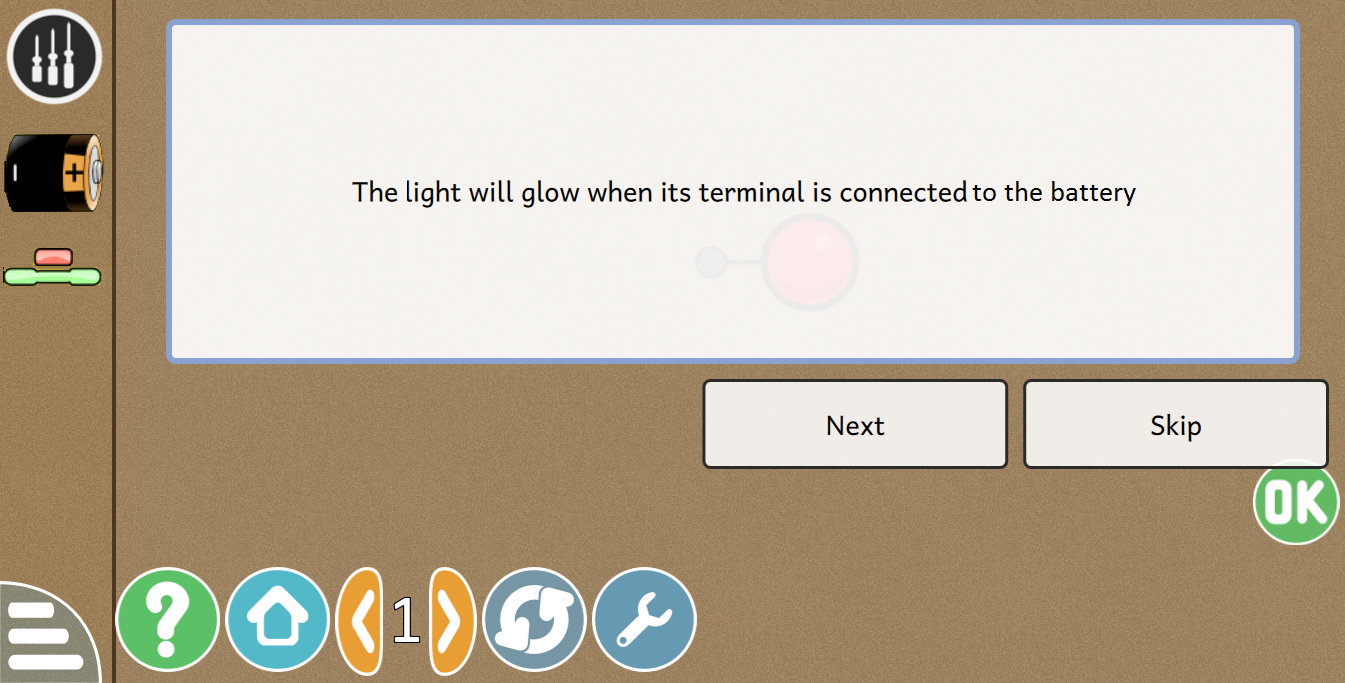
\includegraphics[width=0.9\linewidth]{./images/gsoc1}
			\caption{Mockup for possible layout}
			\end{figure}
						
			\item[$\square$] {So, two separate modes shall be created, where in one, i.e. the tutorial mode, the child can be guided through each tutorial, teaching him/her the basics of analog circuits and components. In the free play mode, the child can then use their new-found knowledge to construct circuits. Some ideas on the modes are:}
			
					\begin{itemize}
					\item {In the initial levels, children will be introduced to the two sources of current, and how can they observe and relate to it in real life. For a DC source, a simple dry cell will be used, and for AC, a plug analogous to ones in our homes can be used.}
					
					\item {They will use the above sources in a circuit and see how it works. Separate levels shall be dedicated initially to teaching how the sources work and how they differ. The arrows showing direction of current shall be very helpful in this case. In later levels, both sources shall be kept(in separate levels) to teach them how components work with each source.}
					
					\item {In higher levels, as components like capacitors, solenoids are introduced, they can be taught about what to expect when connected with the two sources. The ‘why’s’ and ‘how’s’ of it can be left out since it will need a lot more than primary school knowledge to understand.}
					
					\item {For components utilising magnetic properties of current like solenoids, children will be taught about the relation between current and magnetism(tutorial on magnetism explained later).}
					
					\item {The free mode will contain all of the components discussed here for free implementation, experimentation and learning of the child. Levels won’t be necessary here.}
					
					\item {For showing the resistance, current and voltage flowing across circuits, Kirchoff’s law will be used. Each component shall have separate functions to keep track of individual current flowing through it. Using that, the overall resistance, current and voltage in the circuit can be calculated. Details of the calculation will be beyond the comprehension of the children, and hence hidden from users.}

					\item {A resistor can be explained analogous to a water tap, which can  restrict/allow water flow.}
					
					\item {Capacitors can be explained as components having a “capacity” to hold current, and how they work with DC and AC. Capacitors shall be made to be used with a dry cell as well as an AC source(a plug) and a resistor in tutorial mode, and the child will be free to experiment in free play.}
					
					\item {For teaching magnetism and why it occurs in current-carrying components, a superficial explanation will be quite helpful. In the tutorials, a magnet can be depicted to be attracting iron nails kept nearby. Children will be encouraged to try out using small magnets and iron objects(under adult supervision of course).}
					
					\item {A solenoid shall be implemented in the same level as above-mentioned tutorial, and hence would need some graphical cues, like when a solenoid is switched on, some nearby iron nails will be animated to move(attracted) towards it, and stick to it, thus displaying magnetic behaviour. The solenoid is being introduced only to teach that current can produce magnetism, and its applications in real life.}					
					
					\end{itemize}
			\end{itemize}
			
			\begin{figure}[H]
			\centering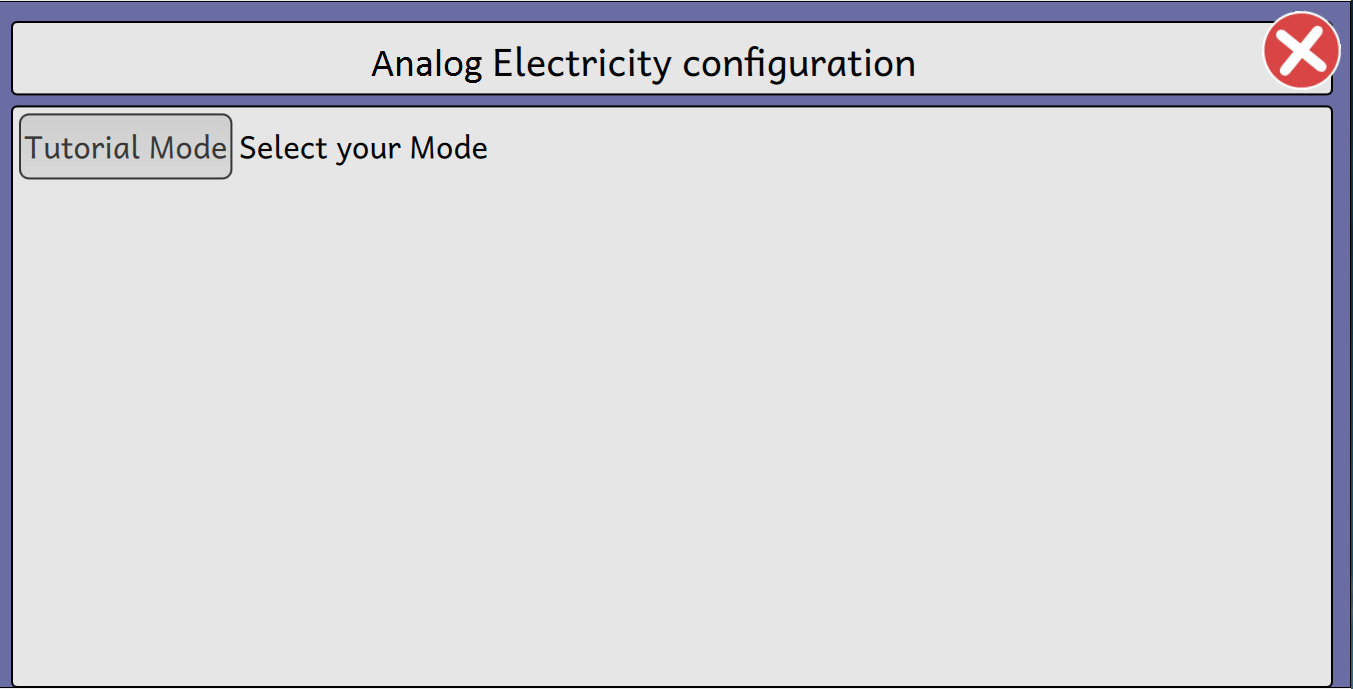
\includegraphics[width=0.9\linewidth]{./images/gsoc2}
			\caption{Mockup for modes}
			\end{figure}
			
			\begin{figure}[H]
			\centering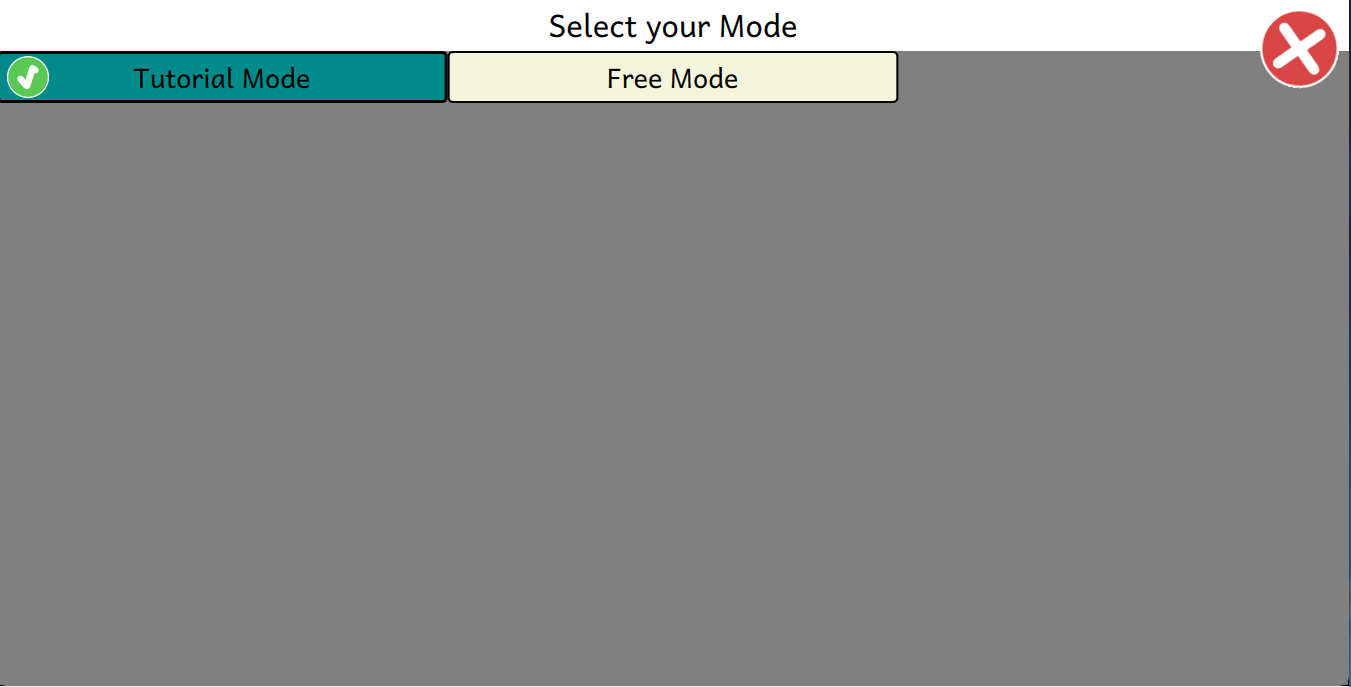
\includegraphics[width=0.9\linewidth]{./images/gsoc3}
			\caption{Mockup for choice between modes}
			\end{figure}
			
			\item[$\blacksquare$] \textbf{Simulator for analog components and circuits:}
				\begin{itemize}
				\item[$\square$] {A sandbox for making circuits and testing out components will be created, which will enable adding/removing components, connecting various circuits and testing them out.}
				\item[$\square$] {Components will be modeled as closely as possible to represent how they actually look and work in real life. Unlike digital electronic components, which work on discrete values, analog components shall be modeled to work with any voltage values and give correct or close to correct results. Clicking on them will show their names, and tutorials shall show how they work.}
				
				\begin{figure}[H]
				\centering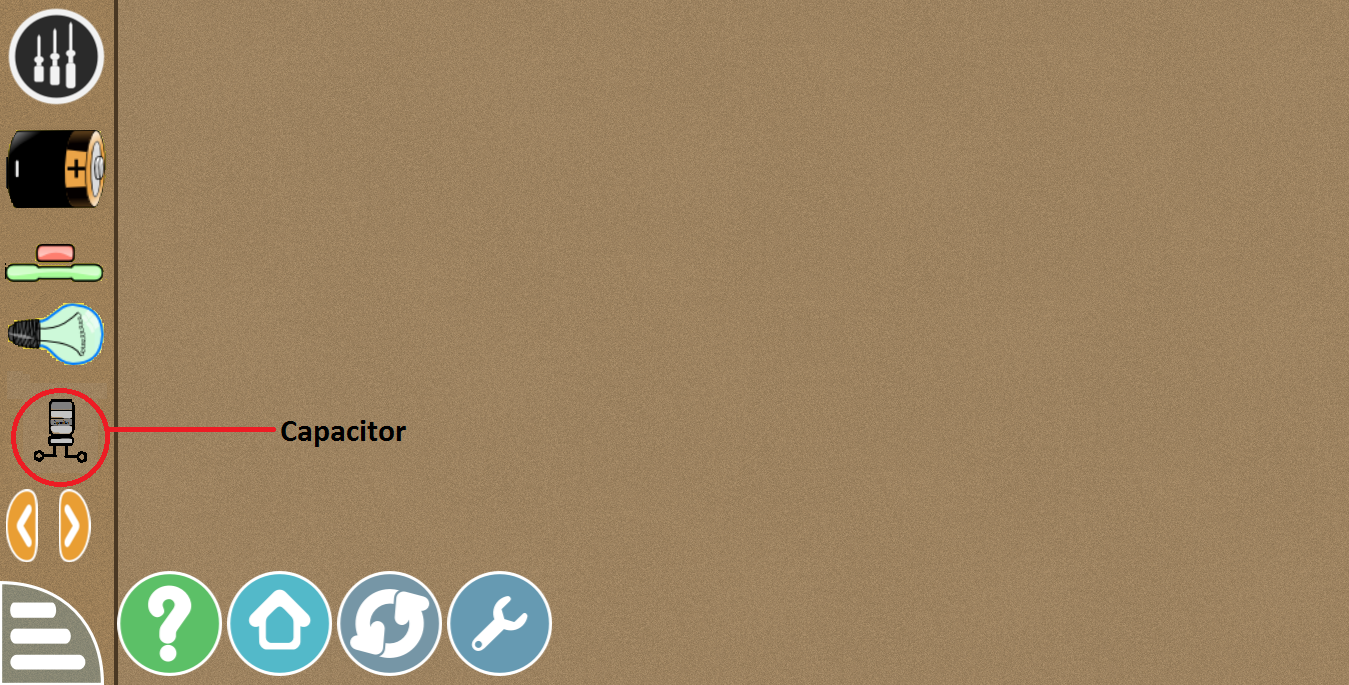
\includegraphics[width=0.9\linewidth]{./images/gsoc4}
				\caption{Mockup showing pinchArea and components}
				\end{figure}
			
				\item[$\square$] {The external library, available at \href{https://github.com/Aerlinger/maxwell}{https://github.com/Aerlinger/maxwell}, although implements various analog components, cannot be directly used here, as Qt Quick does not support js classes. So this library shall be solely used for technical lookups and taking ideas on how to better implement components. Most of the ideas below have been formulated after a thorough observation of the repository.}
				
					\begin{itemize}
					\item {Since js classes aren’t available in Qt, each component will be implemented with its own separate js file, and exported as a module to be used in circuits.}
					
					\item {A base circuit component file shall be shared among all other components, containing basic features like resistance, voltage, etc. and functions to calculate the values of the attributes, as well as rendering them on screen.}
					
					\item {The interface shall be similar to digital electricity, easy for children to interact and understand.}
					
					\item {For the oscilloscope, Qt Charts can be used(optional: may be configured to use OpenGL for rendering waveforms in OpenGL devices). The other options are:}
					
						\begin{itemize}
							\item {Using smoothie (\href{http://smoothiecharts.org/}{http://smoothiecharts.org/})(js charting library)}
							
							\item {Using d3.js (\href{https://d3js.org/}{https://d3js.org/}) along with Qml to render graphs(the external library uses d3.js and rickshaw (\href{https://www.npmjs.com/package/rickshaw}{https://www.npmjs.com/package/rickshaw}), relying on d3.js).}
						\end{itemize}					
					
					\item {As in the external library, we can use marquee text to denote the direction of flow of current, with different colours for various directions of current flow, or determine the direction of current by the polarity of the source, and assign simple arrows at the ends of connections(later option looks better).}\\
					\end{itemize}
					
					\item[$\square$] {Lastly, all of the components(js files, including wires) shall be brought together using Qml.}			
				\end{itemize}
				
				\begin{figure}[H]
				\centering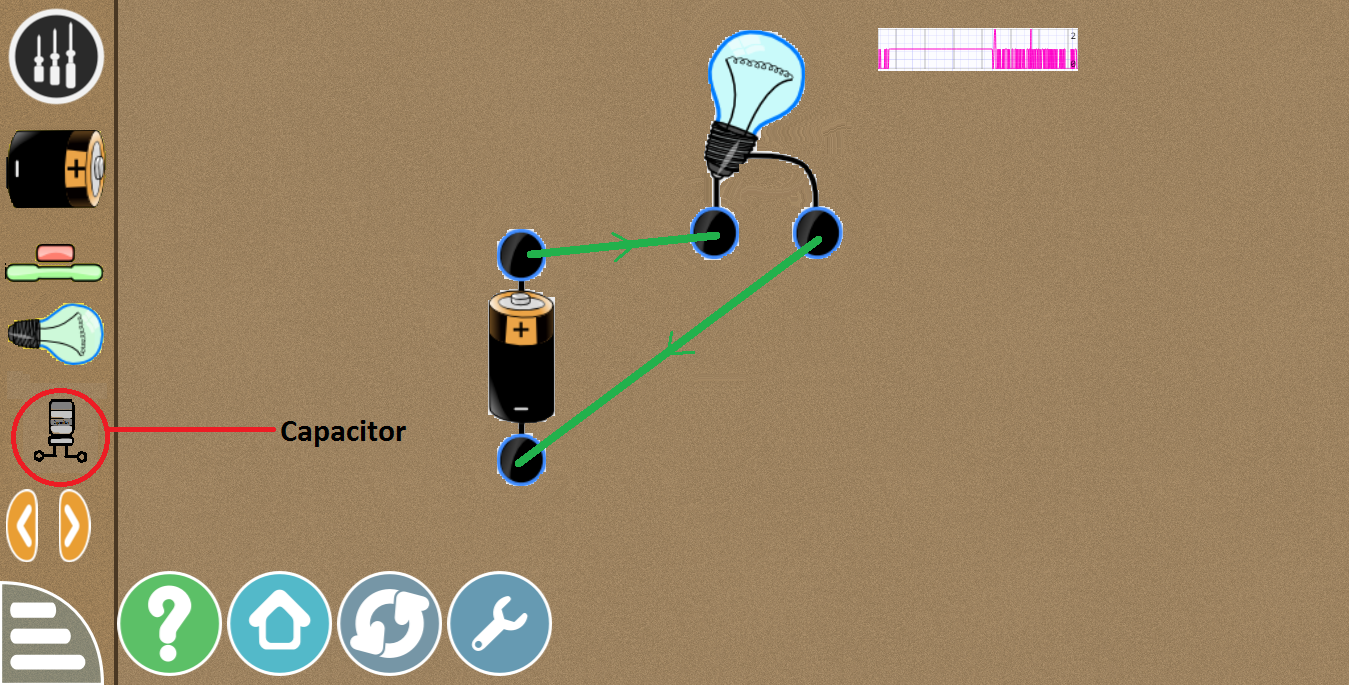
\includegraphics[width=0.9\linewidth]{./images/gsoc5}
				\caption{Mockup showing circuits with current direction and waveform}
				\end{figure}
				
		\item[$\blacksquare$] \textbf{Add more components:}
			
			\begin{itemize}
			\item[$\square$] {Components like capacitors and solenoids will be added for improved and advanced knowledge on important analog components.}
			
			\item[$\square$] {Addition of components like capacitors, etc. may also be made interesting by adding a simple pre-adjusted oscilloscope(since the children will need a separate tutorial to handle the controls) to show how the waves of an analog signal varies, and a speaker can be added for audio to show how waves sound, with a volume slider.}
			\end{itemize}
			
		\item[$\blacksquare$] \textbf{Improvements in UI:}
			\begin{itemize}
			\item[$\square$] {For the layout, keeping it similar to that of digital electricity will help children easily understand how both are or aren’t related and help them differentiate between them. The dark background will also help in clearer depiction of images and text.}
			\item[$\square$] {Displaying voltage, current in case of power source and bulbs, and resistance as well in case of resistors, etc. under the components rather than on them.}
			
			\item[$\square$] {Using a darker background to enable better legibility of text displayed.}
			
			\item[$\square$] {Wires to show arrows to display direction of current flow(helpful in case of capacitors, etc.)}
			
			\item[$\square$] {To prevent cluttering of various components as levels increase, pinchArea shall be implemented to enable navigation among various components in free mode.}\\
			\end{itemize}
			
		\item[$\blacksquare$] \textbf{Increasing difficulty with levels:}
			\begin{itemize}
			\item[$\square$] {Levels shall be presented in tutorial mode only, so that children can get help to progressively learn the various components and their functions. In free mode, all components shall be available for practice and experimentation.}
			
			\item[$\square$] {Components mentioned earlier will be introduced into the activity at a much later stage, since these will require a much thorough knowledge even for using in a basic circuit.}
			\end{itemize}
		\end{itemize}
\bigskip\bigskip

\section{Timeline}
\label{S:1}

\begin{center}
\setlength{\extrarowheight}{1.75pt}
\begin{tabularx}{\linewidth}{|l|X|}
\hline

\textbf{Time Period} & \textbf{Activity for the Period}\\
\hline

{April 24 - August 14, 2018} & {\textit{Analog Electricity}}\\
\hline

{April 24 - May 13} & {\textit{Community Bonding}}\\
\hline

 & \par
\parbox{12cm}{
\begin{itemize}[noitemsep, topsep=2pt]
	\item Bond with the mentors, go through further documentation and look up useful libraries.
	\item Take notes and suggestions from mentors and bond with other GSoC candidates.
\end{itemize}
}\\
\hline\hline

{May 14 - June 12} & {\textit{Development of Basic Layout and Simulator}}\\
\hline

{May 14 - May 20} & \par
\parbox{12cm}{
\begin{itemize}[noitemsep, topsep=2pt]
	\item Build the basic main layout and layouts for tutorial and free mode, similar to digital electricity, without components(generalize code between activities as much as possible)
\end{itemize}
}\\
\hline

{May 21 - May 24} & \par
\parbox{12cm}{
\begin{itemize}[noitemsep, topsep=2pt]
	\item Submit work for review
	\item Add improvements based on suggestions
\end{itemize}
}\\
\hline

{May 25 - June 10} & \par
\parbox{12cm}{
\begin{itemize}[noitemsep, topsep=2pt]
	\item Test out codes from external libraries, and start implementing basic components without classes

	\begin{itemize}[noitemsep, topsep=2pt]
		\item Using json files to depict various features of components like voltage, resistance,etc will make it easier to handle and change while development and testing(much like in the external library)
		
		\item Functioning of components will be better handled by separate js files for each type of component(initially implementing simple ones like resistors)
		
		\item Basic components like bulbs, small resistors, switches, potentiometers and DC sources shall be implemented, using simple circuits.
	\end{itemize}
\end{itemize}
}\\
\hline

{June 11 - June 12} & \par
\parbox{12cm}{
\begin{itemize}[noitemsep, topsep=2pt]
	\item Submit work for possible improvements before final submission for phase 1 review
\end{itemize}
}\\
\hline\hline

{June 13 - June 15} & {\textit{Submission and Review - Phase I
}}\\
\hline

 & \par
\parbox{12cm}{
\begin{itemize}[noitemsep, topsep=2pt]
	\item Submit work for review by mentors
	\item Make changes as suggested in reviews
	\item Submit work for final evaluation of Phase I
\end{itemize}
}\\
\hline\hline

{June 16 - July 10} & {\textit{Addition of tutorials and advanced components
}}\\
\hline

{June 16 - June 25} & \par
\parbox{12cm}{
\begin{itemize}[noitemsep, topsep=2pt]
	\item Work on developing tutorials easy enough to be understood by children. The tutorials shall be built first so as to give an insight on how to proceed to make future components next.

	\begin{itemize}[noitemsep, topsep=2pt]
		\item Tutorials for resistors shall consist of pictures depicting what and why of a resistor, followed by how to use them, and analogies to taps being used to restrict water flow similar to resistors restricting current flow.
		
		\item Concepts of serial and parallel circuits shall be introduced next. Levels shall be particularly allotted for this purpose.
		
		\item For capacitors, children shall be taught what a capacitor does, i.e. store electricity, and hence how it is different from  a battery. A simple circuit can be depicted in images, consisting of a bulb which will slowly dim out on disconnecting from a DC cell, as it will be connected to a capacitor in parallel.

	\end{itemize}
\end{itemize}
}\\
\hline

 & \par
 \parbox{12cm}{
	\begin{itemize}[noitemsep, topsep=2pt]
		\item[] 
		\begin{itemize}[noitemsep, topsep=2pt]
			\item For solenoids, a tutorial level will be included where magnetism will be exhibited as follows: a solenoid connected with a battery will be shown. An image of iron nails kept nearby shall be animated to move nearer the solenoid, depicting attraction. In the tutorial, a brief description of a magnet and why it attracts only certain materials.
		\end{itemize}
	\end{itemize}	 
 }\\
 \hline

{June 26 - July 1} & \par
\parbox{12cm}{
\begin{itemize}[noitemsep, topsep=2pt]
	\item Submit above work for review
	\item Discuss possible improvements and fixes
\end{itemize}
}\\
\hline

{July 2 - July 9} & \par
\parbox{12cm}{
\begin{itemize}[noitemsep, topsep=2pt]
	\item Work on modelling additional components like capacitors as well as increase levels and their difficulty.
	
	\begin{itemize}
		\item Start working on AC source and capacitors(partial implementation)
	\end{itemize}
\end{itemize}
}\\
\hline\hline

{July 10  - July 13} & {\textit{Submission and Review - Phase II
}}\\
\hline

 & \par
\parbox{12cm}{
\begin{itemize}[noitemsep, topsep=2pt]
	\item Submit work for review by mentors
	\item Make changes as suggested and submit for evaluation in Phase II.
\end{itemize}
}\\
\hline\hline

{July 14 - August 7} & {\textit{Final touches to Analog activity
}}\\
\hline

 & \par
\parbox{12cm}{
\begin{itemize}[noitemsep, topsep=2pt]
	\item Complete implementing capacitors.
	\item Implement solenoids(and possibly, oscilloscope and speaker).
	\item Occasional submission of code for review and suggested improvements.
	\item Fixing further issues and implementing final suggestions
\end{itemize}
}\\
\hline\hline

{August 8 - August 14} & {\textit{Submission for final evaluation
}}\\
\hline

 & \par
\parbox{12cm}{
\begin{itemize}[noitemsep, topsep=2pt]
	\item Submission of entire work for final review and suggestions
	\item Handing over final works for evaluation
\end{itemize}
}\\
\hline\hline

\end{tabularx}
\end{center}
\bigskip\bigskip

\section{About Me}
\label{S:1}
{I am currently in my final year at Maulana Abul Kalam Azad University of Technology (formerly WBUT), Kolkata, pursuing B. Tech. in Computer Science and Engineering. I have been contributing to the Qt version of GCompris since September 2017. Some of my contributions are:}
\begin{itemize}
\item {Removed dependency of ball direction on mouse buttons in Penalty activity:\\
\href{https://cgit.kde.org/gcompris.git/commit/?id=c94d7454c5a05364a1cbeae5b0bd1bed552ae5ed}{https://cgit.kde.org/gcompris.git/commit/?id=c94d7454c5a05364a1cbeae5b0bd1bed552ae5ed}}

\item {Progress bar corresponding to click zone only will be animated in Penalty activity:\\
 \href{https://cgit.kde.org/gcompris.git/commit/?id=e5b68f68657cf1ac25a6aa31924acfaf4a180f0b}{https://cgit.kde.org/gcompris.git/commit/?id=e5b68f68657cf1ac25a6aa31924acfaf4a180f0b}}

\item {Added easy mode in Letter-In-Word activity:\\
\href{https://cgit.kde.org/gcompris.git/commit/?id=c48f7057c27166edc6b8297bb3518a10ec2ee31b}{https://cgit.kde.org/gcompris.git/commit/?id=c48f7057c27166edc6b8297bb3518a10ec2ee31b}}

\item {Improved layout in Hangman activity:\\
\href{https://cgit.kde.org/gcompris.git/commit/?id=6a66cd44106015bd369616574d656a8dd19d15be}{https://cgit.kde.org/gcompris.git/commit/?id=6a66cd44106015bd369616574d656a8dd19d15be}}

\item {Fixed coding style issues for Ascending-Order activity:\\
\href{https://cgit.kde.org/gcompris.git/commit/?id=ade955e042ceb9774459a1181382159606a31502}{https://cgit.kde.org/gcompris.git/commit/?id=ade955e042ceb9774459a1181382159606a31502}}

\item {Added option to change case of letter to find in Letter-In-Word activity:\\
\href{https://commits.kde.org/gcompris/7c769594a5372e560904511404e2d1e156904050}{https://commits.kde.org/gcompris/7c769594a5372e560904511404e2d1e156904050}}
\end{itemize}
\bigskip
\textbf{Website: }\href{mouri11.github.io}{mouri11.github.io}\\
\textbf{Contact Info:}\\
\textbf{Email: }{rohit.das950@gmail.com}\\
\textbf{IRC Nick: } mouri11

\end{document}

%%
%% End of file `elsarticle-template-1-num.tex'.
